\documentclass[oneside,14pt]{extarticle}
\usepackage{cmap}
\usepackage[utf8]{inputenc}
\usepackage[english,ukrainian]{babel}
\usepackage{graphicx}
\usepackage{geometry}
\usepackage{listings}
\usepackage{float}
\usepackage{amsmath}
\usepackage{subfig}
\usepackage{tempora}
\geometry{
	a4paper,
	left=20mm,
	right=20mm,
	top=15mm,
	bottom=15mm,
}
\lstset{
	language=c,
	tabsize=4,
	keepspaces,
	showstringspaces=false,
	frame=single,
	breaklines,
	language=C,
}
\graphicspath{ {./pictures} }
\setlength{\parindent}{4em}

\newcommand\subject{Системне адміністрування}
\newcommand\lecturer{професор кафедри ПЗ\\Фечан А.В.}
\newcommand\teacher{професор кафедри ПЗ\\Фечан А.В.}
\newcommand\mygroup{ПЗ-42}
\newcommand\lab{4}
\newcommand\theme{Реалізація механізму групових політик у Windows 10. Аналіз
	і налаштування безпеки}
\newcommand\purpose{Ознайомлення зі структурою, принципом роботи та
	налаштуванням об’єкта групової політики на локальному комп’ютері під
	управлінням ОС Windows 10. Навчитись використовувати та створювати
	шаблони безпеки для ефективного налаштування та аналізу типових параметрів
	безпеки}

\begin{document}
\begin{normalsize}
	\begin{titlepage}
		\thispagestyle{empty}
		\begin{center}
			\textbf{МІНІСТЕРСТВО ОСВІТИ І НАУКИ УКРАЇНИ\\
				НАЦІОНАЛЬНИЙ УНІВЕРСИТЕТ "ЛЬВІВСЬКА ПОЛІТЕХНІКА"}
		\end{center}
		\begin{flushright}
			\textbf{ІКНІ}\\
			Кафедра \textbf{ПЗ}
		\end{flushright}
		\vspace{80pt}
		\begin{center}
			\textbf{ЗВІТ}\\
			\vspace{10pt}
			до лабораторної роботи № \lab\\
			\textbf{на тему}: <<\textit{\theme}>>\\
			\textbf{з дисципліни}: <<\subject>>
		\end{center}
		\vspace{80pt}
		\begin{flushright}
			
			\textbf{Лектор}:\\
			\lecturer\\
			\vspace{28pt}
			\textbf{Виконав}:\\
			
			студент групи \mygroup\\
			Коваленко Д.М.\\
			\vspace{28pt}
			\textbf{Прийняв}:\\
			
			\teacher\\
			
			\vspace{28pt}
			«\rule{1cm}{0.15mm}» \rule{1.5cm}{0.15mm} 2024 р.\\
			$\sum$ = \rule{1cm}{0.15mm}……………\\
			
		\end{flushright}
		\vspace{\fill}
		\begin{center}
			\textbf{Львів — 2024}
		\end{center}
	\end{titlepage}
		
	\begin{description}
		\item[Тема.] \theme.
		\item[Мета.] \purpose.
	\end{description}

    \section*{Лабораторне завдання}
	\begin{enumerate}
		\item Відкрити оснащення mmc "Group Policy". Перейти в гілку "Password
		Policy", задати мінімальну довжину пароля. Після цього
		спробувати змінити власний пароль на такий, довжина якого менша за вказану в
		політиці, переконатись в неможливості такої дії. Повторити такі дії з
		параметрами "Password must meet complexity requirements" та "Store passwords
		using reversible encryption".
		\item Перейти в гілку "Account lockout threshold", задати граничне
		значення блокування. Після цього спробувати декілька разів зайти в
		систему з неправильним вводом пароля – переконатись у спрацюванні
		блокування. Увійти в систему як адміністратор – зняти блокування
		вручну з оснастки "Local Users and Groups" у властивостях заблокованого
		облікового запису.
		\item Перейти в гілку "Software Restriction Policies". Створити
		нову політику. Не змінюючи політики за замовчуванням створити нове правило
		(правила), що забороняє виконання програм з будь-якого тому крім "С:" (при
		потребі створити логічні диски або розділи). Спробувати виконати
		будь-який файл з цього тому. Створити нове правило для хешу
		програми, яке дозволить виконувати саме цей вказаний файл.
		Спробувати запустити на виконання цей файл.
		\item Відкрити оснастку mmc "Security Configuration and Analysis" . Створити нову базу даних, яка буде відображати стан налаштування політик
		комп’ютера за певним шаблоном.
	\end{enumerate}

	\section*{Хід роботи}
	
	\begin{figure}[H]
		\centering
		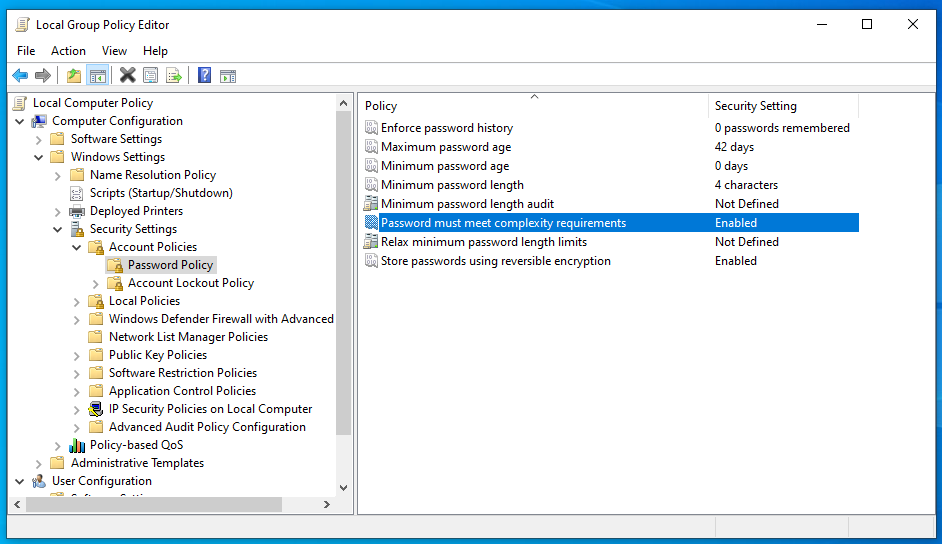
\includegraphics[width=\columnwidth]{1}
		\caption{Встановлення групової політики для паролів}
	\end{figure}
	
	\begin{figure}[H]
		\centering
		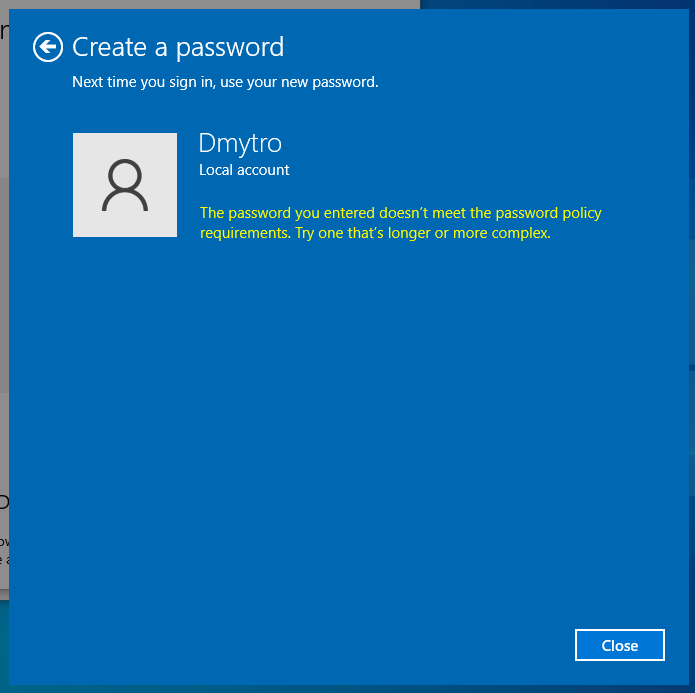
\includegraphics[width=\columnwidth]{2}
		\caption{Результат встановлення групової політики для паролів}
	\end{figure}
	
	\begin{figure}[H]
		\centering
		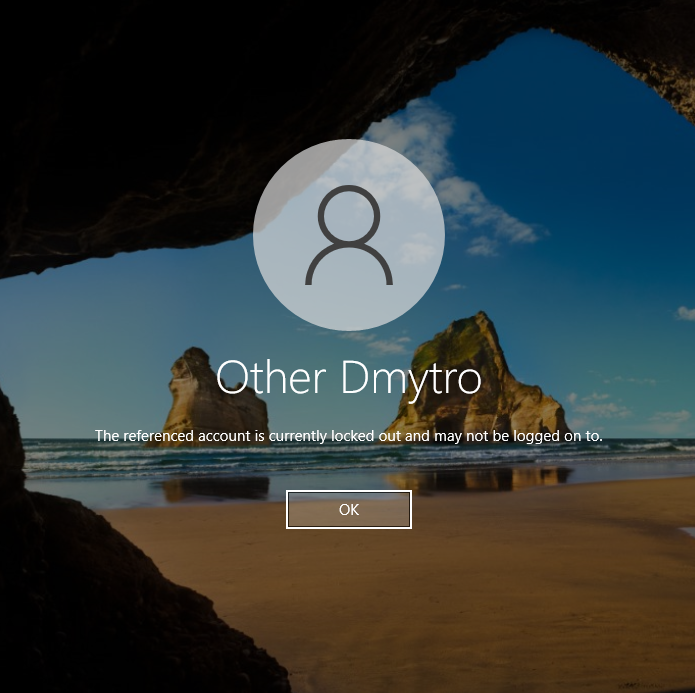
\includegraphics[width=\columnwidth]{3}
		\caption{Результат встановлення групової політики для паролів}
	\end{figure}
	
	\begin{figure}[H]
		\centering
		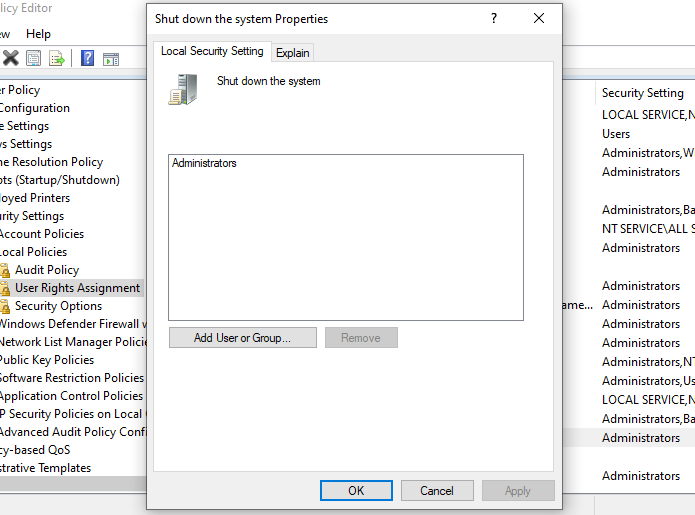
\includegraphics[width=\columnwidth]{4}
		\caption{Встановлення групової політики на заборону вимкнення}
	\end{figure}
	
	\begin{figure}[H]
		\centering
		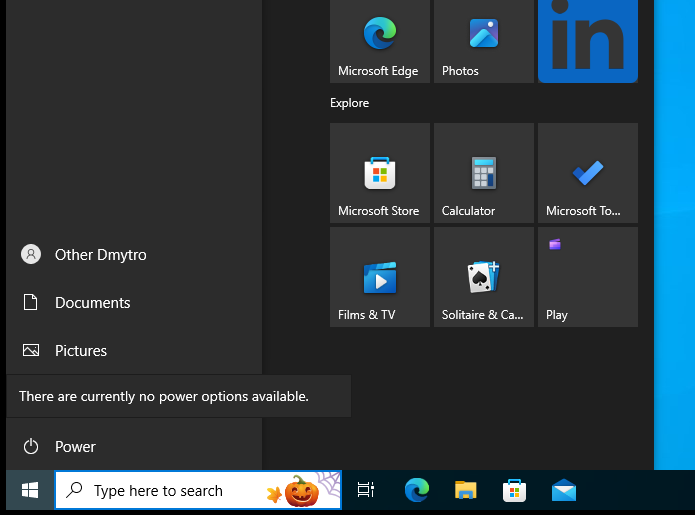
\includegraphics[width=\columnwidth]{5}
		\caption{Результат встановлення групової політики}
	\end{figure}
	
	\begin{figure}[H]
		\centering
		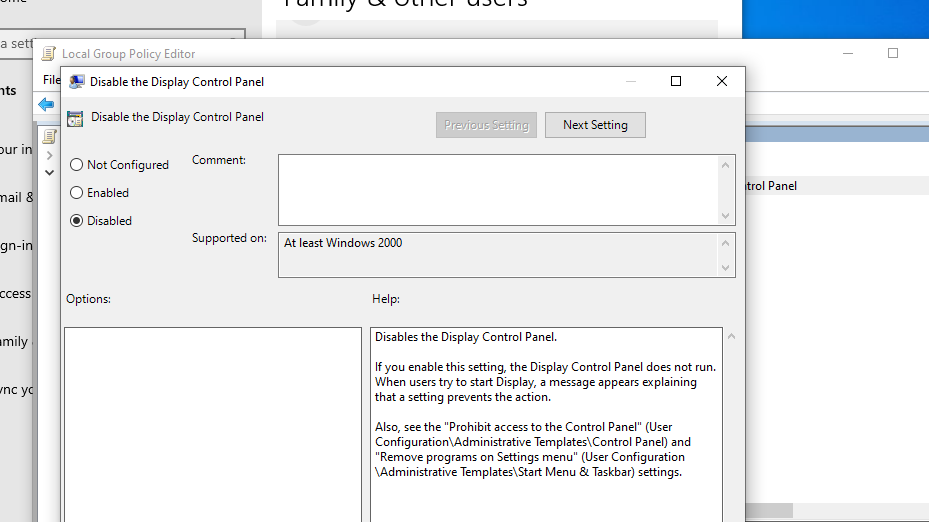
\includegraphics[width=\columnwidth]{6}
		\caption{Встановлення групової політики}
	\end{figure}
	
	\begin{figure}[H]
		\centering
		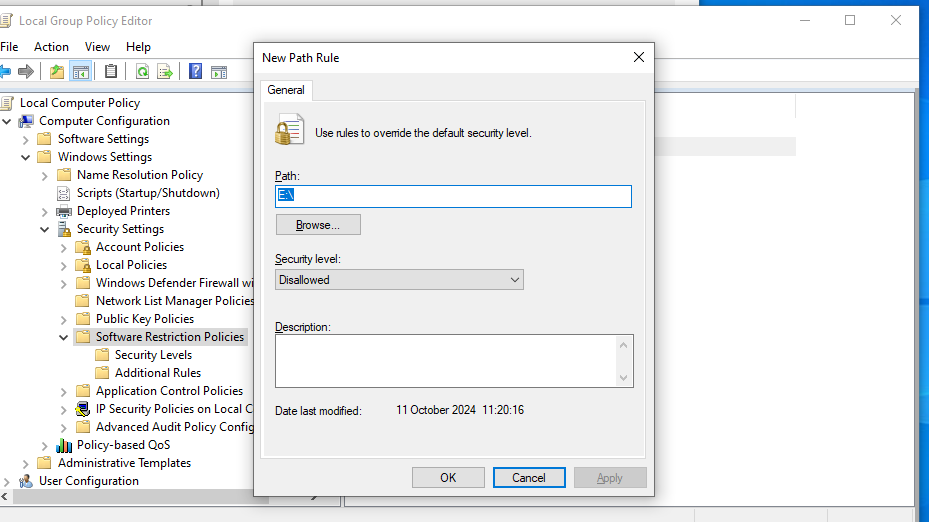
\includegraphics[width=\columnwidth]{7}
		\caption{Встановлення групової політики}
	\end{figure}
	
	\begin{figure}[H]
		\centering
		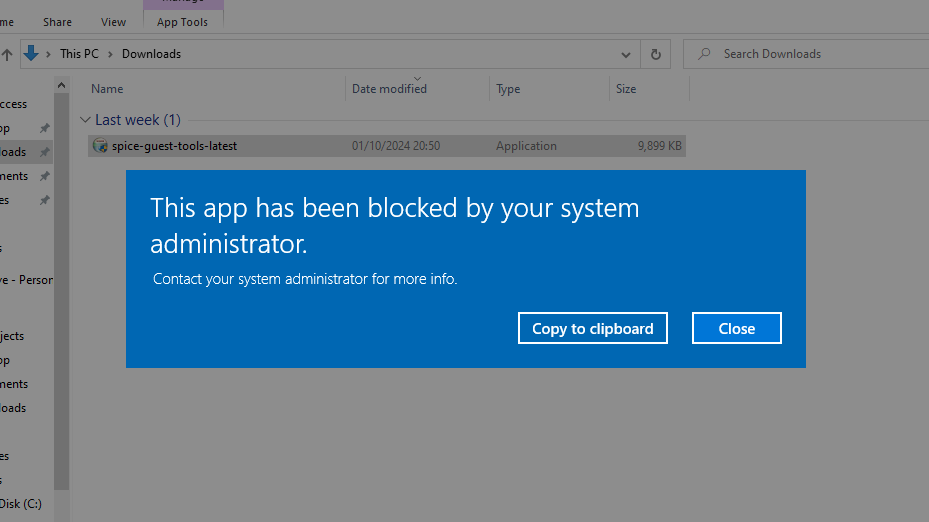
\includegraphics[width=\columnwidth]{8}
		\caption{Результат встановлення групової політики}
	\end{figure}
	
		\begin{figure}[H]
		\centering
		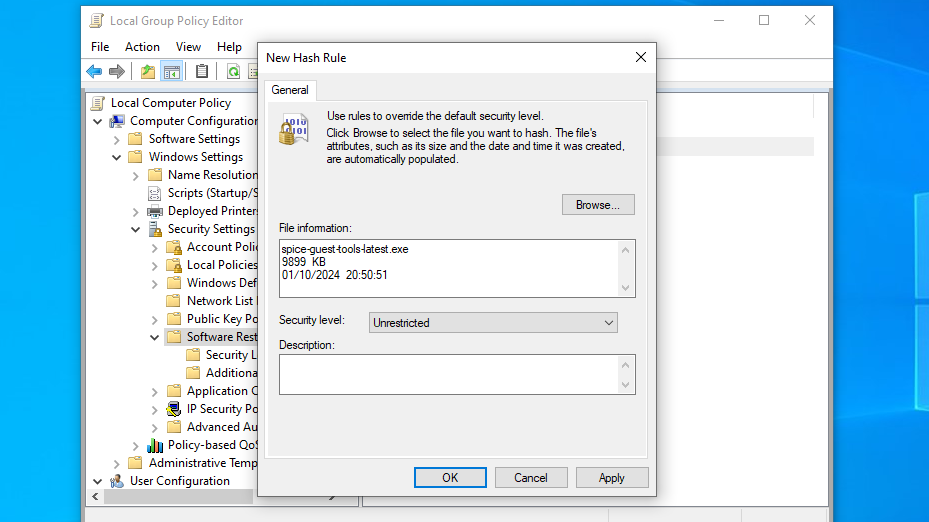
\includegraphics[width=\columnwidth]{9}
		\caption{Встановлення групової політики}
	\end{figure}
	\begin{figure}[H]
		\centering
		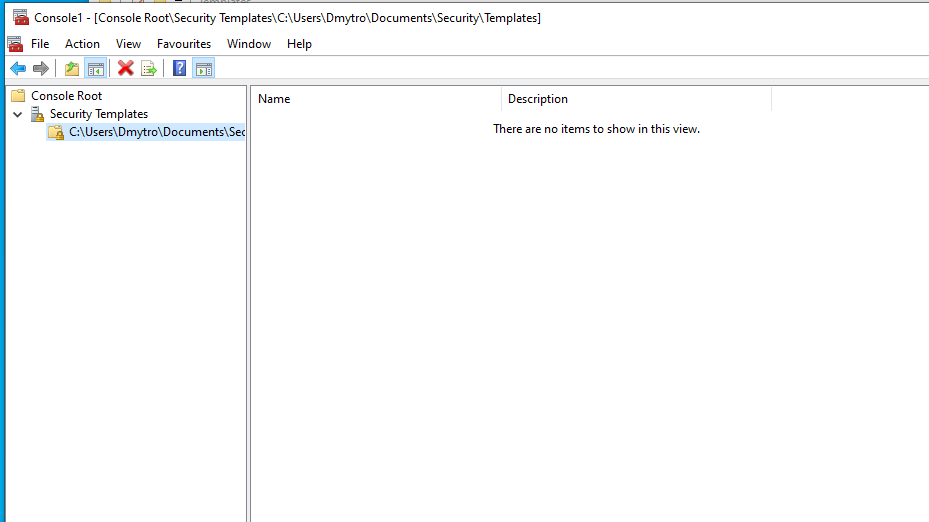
\includegraphics[width=\columnwidth]{10}
		\caption{Встановлення шаблону}
	\end{figure}
	
	\section*{Висновки}
	Під час виконання лабораторної роботи я ознайомився зі структурою, принципом роботи та
	налаштуванням об’єкта групової політики на локальному комп’ютері під
	управлінням ОС Windows 10. Навчився використовувати та створювати
	шаблони безпеки для ефективного налаштування та аналізу типових параметрів
	безпеки.
		    
\end{normalsize}
\end{document}
